
%
% Incomplete latex outline translated from three.docx.  That outline is official.
%

\chapter{Zero-mode Signal Instrumentation}

\begin{bf}
\author{  
L. J. Greenhill 
(Harvard-Smithsonian Center for Astrophysics) \\
R. Subrahmanyan 
(Raman Research Institute)   
}\\



\noindent
Experiments that seek to detect a sky-averaged (zero-mode) HI signature during the Epoch of Reionization and Cosmic Dawn use purpose-built instrumentation that is elementary in concept (e.g., dipole antennas and spectrometers) but subtle in design owing to exceptional calibration tolerances.  This chapter presents the rudiments of radiometry, discussion of instrument design and calibration, and in the process, describes design approaches for three ongoing experiments: EDGES, SARAS, and LEDA. \\

\end{bf}

\section{Introduction}

Several experiments have been deployed to measure predicted sky-averaged or zero-mode signals from HI at redshifts ($z$) from approximately 7 to 23 (180 to 60 MHz). The {\underline E}xperiment to {\underline D}etect the {\underline G}lobal {\underline E}OR {\underline S}ignature (EDGES) \cite{bowman08,rogers12} provided the first constraint on reionization, excluding substantial change in neutral fraction over an interval narrower than $\Delta z\sim 0.06$, with 95\% confidence, for $z\lesssim11)$. Two more experiments, the {\underline B}roadband {\underline I}nstrument for {\underline G}lobal {\underline H}ydrogen {\underline R}eionization {\underline S}ignal--BIGHORNS \cite{sokolowski15}, and the {\underline S}haped (\underline A)ntenna Measurement of the Background {\underline Ra}dio {\underline S}pectrum--SARAS \cite{patra13, singh17, singh18} also sought to constrain parameters describing reionization.  SARAS~2 excluded some parameter combinations corresponding to late X-ray heating and rapid reionization, with 68 to 95\%.  
% Ravi to LJG: To my knowledge, BIGHORNS did not constrain parameters describing reionization; I suggest we drop their mention above.

Several experiments also target setting constraints on parameters describing conditions during Cosmic Dawn (CD) through detection of the predicted HI absorption against the Cosmic Microwave Background (CMB), which may be more readily separated from foreground contamination than the EOR signal owing to narrowness in redshift, in many models.  Exploiting techniques and radio-frequency (RF) electronics refined during  preceding work at lower redshift, EDGES has claimed detection of a trough \cite{bowman18} though with unlikely fitted amplitude, breadth, and shape.  As of this writing, much needed independent confirmation is pending \cite{greenhill18,hills18,bradley19,spinelli19}.  The SARAS~3 high-redshift ($15\lesssim z \lesssim 25$) successor experiment \cite{singh17,singh18} has collected data with multiple antenna architectures and at widely separated sites.  The {\underline L}arge-aperture {\underline E}xperiment to Detect the {\underline D}ark {\underline A}ge -- LEDA \cite{greenhill12,price18}, uses several configurations of the standard antenna first engineered by the Long Wavelength Array (LWA) project \cite{taylor12} and embeds them in a dense interferometric array to make possible calibration techniques  unavailable for standalone antennas.  SCI-HI \cite{voytek14}, and  the related {\underline P}robing {\underline R}adio {\underline I}ntensity at High $z$ from {\underline M}arion island (PRIZM) experiment \cite{philip19}, achieving early data at two of the most radio quiet sites used thus far (e.g., judged from limited FM radio contamination), while following similar methodologies and instrumentation approaches.
% Ravi to LJG: I suggest we drop the references \cite{singh17,singh18} from the above para, where reference is to SARAS 3 that is operating in the 50-100 MHz band.

\
\begin{figure}[htb]
\begin{center}
\hspace*{-0.15in}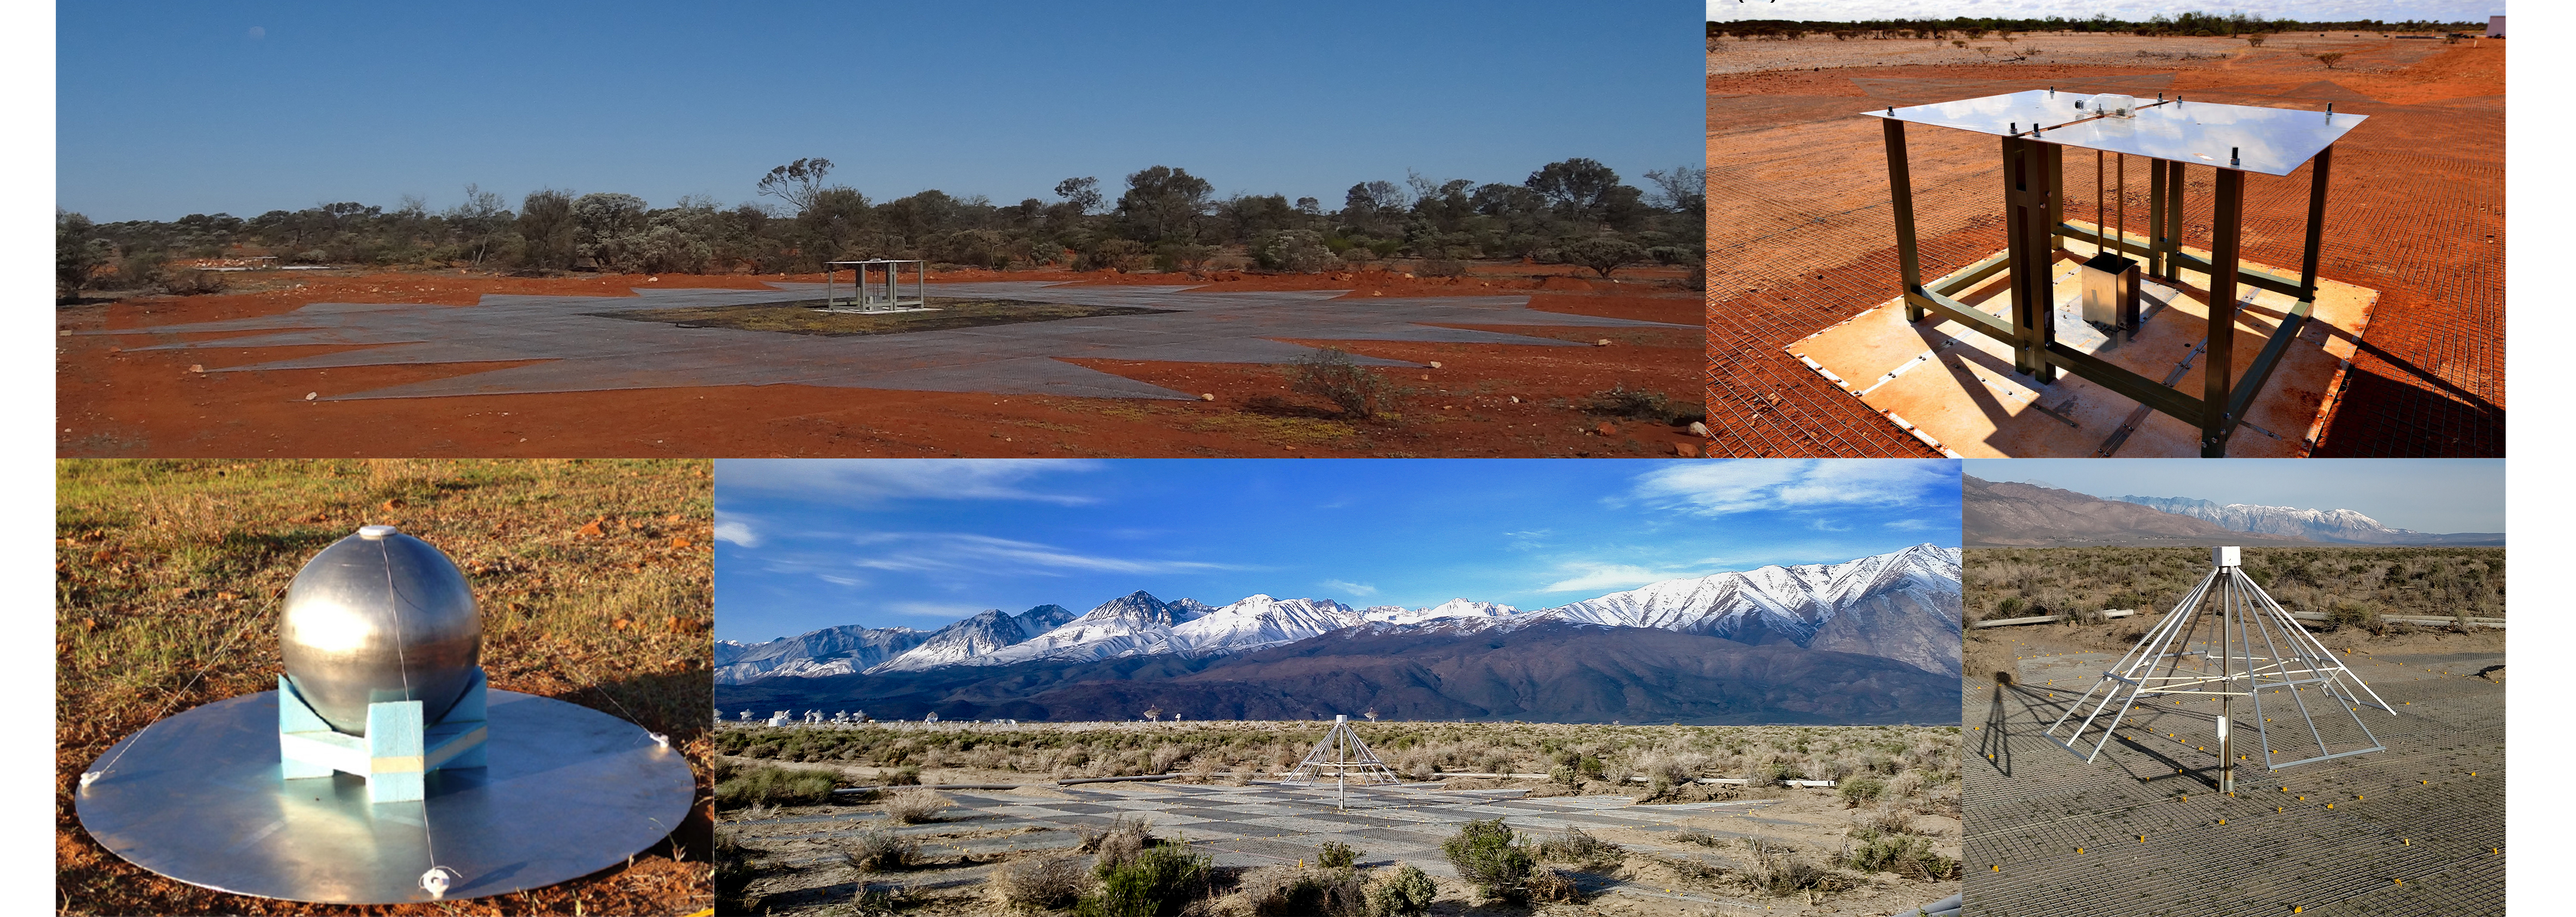
\includegraphics[width=1.05\textwidth]{EDGES_SARAS_LEDA_figure_19sep20.jpg}
\end{center}
\caption{(top left) EDGES antenna and serrated 30~m $\times$ 30~m ground screen.  (top right) Closeup of the EDGES single polarization dipole comprising two metal squares.  (bottom right) Closeup of the LEDA dual polarization pyramidal dipole.  (bottom center) LEDA antenna and serrated 20~m $\times$ 20~m ground screen. (bottom left) SARAS~2 sphere-disc antenna consisting of a spherical element atop a 0.87~m diameter disc.  The maximum gains for EDGES and LEDA antennas are toward zenith.  In contrast, the maximum for SARAS traces a ring on the sky centered on zenith, where there is a null.}
\end{figure}
% RAVI to LJG: I've changed the caption to SARAS 2 antenna somewhat.

% LJG: Consider adding guidance re significant elements that'll be treated later in the cal. §.

\section{Radiometer Basics}

Karl Jansky discovered that any sensor of electromagnetic fields placed beneath open sky samples at its terminals ``cosmic radio noise''\footnote{The term ``noise'' is commonly used because radio frequency (RF) radiation from atomic processes in cosmic sources and terrestrial thermal sources are spatially and temporally incoherent.  The fields are generally described statistically as Gaussian random variables of zero mean, following from the Central Limit Theorem.}  \cite{jansky33}.  A typical channelized radiometer comprises an antenna, an amplifying receiver that includes a band-limiting filter, and a digitizer.  The filter defines the measurement bandwidth.   The digitizer samples data at a rate of twice the bandwidth or faster, thereby enabling use of Fourier techniques to transform time-series into spectra. For an Earth-bound system, that power may include RF emission from the ground proximate to the antenna,  self-generated noise from the electronics (e.g., amplifiers), and artificial terrestrial interference.  For scale, we note that an antenna with unit gain in equilibrium with a 300\,K blackbody delivers a noise power of {\it O}(1)\,pW over a 100\,MHz band.

% N.B.  Use of baseband is unstated.  Explain here or later.

\subsection{Antenna}
  
The simplest form of antenna comprises two oppositely directed conductors (a dipole).  Incident waves induce currents in the conductors and a voltage is developed across the inward facing ends (the terminals). The spectrum of power measurable at the terminals corresponds to the incident waves, modified by the frequency-dependent electromagnetic coupling of the antenna and surrounding space, and the transfer function between the terminals and instrumentation downstream.
  
Antenna geometry determines coupling to the sky, transfer function from antenna to amplifying receiver, and coupling to the ground, which is generally kept low.  A dipole with wire-like arms each of length one quarter wavelength will have a resonance at wavelength $\lambda_\circ$, and in a narrow band, its maximum power transfer efficiency.  In so doing, the antenna acts as a transformer from the impedance of free space on one side to that of transmission lines and RF electronics on the other.  Impedance mismatches reflect power and degrade efficiency, and these increase away from the resonant frequency.
  
Antennas used for CD/EOR radiometry must operate efficiently and usefully over an octave or more in frequency ($\nu_{\rm high}/\nu_{\rm low}=2 or 0.66\Bar{\nu}<\nu<1.33\Bar{\nu})$ in order to distinguish the predicted complex spectral structure due to the 21-cm transition and smoothly varying foregrounds.  Broadband dipoles may be planar with arms comprising 2D shapes (e.g., plates in the case of EDGES), 3D structures with planar arms (e.g., an inverted {\bf V} in the case of LEDA) or more complex structures.  Linear dipoles couple to a single linear polarization mode (oriented along the dipole arms).  Dipoles with spiral and helical arms couple to the circularly polarized mode propagating on axis and jointly to circular and linear modes off axis.
Self-similar planar and conical spirals may have operational bandwidths that exceed an octave and maintain good impedance matching, but other metrics may suffer (e.g., gain pattern variation with frequency or ``chromaticity''). 

\subsubsection{Ground sensitivity}

Owing to its symmetry, a planar dipole receives radiation incident from the sky and ground equally well.  ``Drooping'' or raising the arms of a linear dipole (e.g., SCI-HI) or projecting a spiral onto a cone (e.g., as for BIGHORNS) are common techniques to break the symmetry, narrowing the the field of view and increasing antenna ``directivity.''  However, substantive suppression of coupling to the ground is best achieved by covering the ground with a conducting plane.  The ground ``screen'' acts as a reflector.  The antenna senses the sky above and below, boosting sensitivity for suitable antenna-screen separation (e.g., the direct and reflected paths interfere constructively for $\lambda_\circ$/2 separation ). 
%Ravi to LJG: Should not the antenna-screen separation be $\lambda_\circ$/4? And the constructive interference would be for rays from zenith.

Ground screens may be soldered or welded wire mesh, with minimum conductor spacing or hole size $\ll \lambda_\circ$, so as to minimize leakage of radiation across the plane.  However, reflection and scattering off the discontinuity represented by the edge of the ground screen creates interference patterns that are functions of incident direction and frequency, thereby modulating antenna gain enough that fluctuations in the baseline of a spectrum may be apparent.  Adding a random component to the geometry suppresses the effect to a degree, but at low frequencies, the addition of fractal-like designs {\it O}($\lambda$) in extent, sculpted in wire mesh, is impractical.  Instead, serration is an effective tool, as in Figure 1 (e.g., EDGES, LEDA).

%% LJG notes for later.  Confirm adequate treatment of:
%% -Gain pattern characteristics:  achromatic response. 
%% -Electrically small antennas.  Main lobe. 
%% -Antenna impedance characteristics
%% -Tabulation of desirable characeristics that enable radiometry
%%  Editorial comment to consider -- dipoles are good for X.  For 21cm we use them for Y.

% TEXT REMOVED FOR POSSIBLE USE LATER
 %Just as antennas are frequency selective, so also are antenna selective in their direction sensitivity.  I know of no practical antenna that is isotropic.  The relative sensitivity of an antenna across sky directions is referred to as the far-field antenna radiation pattern or beam pattern.  Any antenna is directional and is selective is receiving radiation. A quarter wave dipole antenna is insensitive to radiation incident along its length: after all, radiation incident along that direction would have fields orthogonal to the dipole arms and hence cannot possibly induce currents.  The quarter wave dipole antenna efficiently transduces signals in directions orthogonal to its orientation: quarter wave dipole antennas have toroidal beam patterns; dipole antennas are omni-directional. The larger an antenna is in its electrical size, the more directional is its response to sky radiation.  Antennas with electrical size exceeding unity would naturally have beam patterns that have a main lobe that defines a sky solid angle where sensitivity is maximum, and sidelobes of lower sensitivity.  Electrically small antennas would have a single main lobe without sidelobes.
  
  %Antennas are usually passive systems, hence reciprocal, and may be viewed as radiators or sensors, transforming incident power to signal power at its terminals or transforming power fed at the terminals to free-space radiation.  The antenna as a transformer provides a transformed free-space impedance at its terminals, which is often referred to as antenna impedance. Viewed as a radiator, power fed to the antenna via a transmission line connected to the antenna terminals is only partly available for radiation, because depending on the impedance mis-match between the transmission line and the antenna a part of the power fed to the antenna is reflected back. Of the power available for radiation, a part of the power flows to sky via the main and side lobes of the radiation pattern, a part to ground via what might be considered to be back lobes and a part might be lost as ohmic loss that heats the antenna, if the conducting antenna elements are resistive.  Reflection efficiency of the antenna defines the fractional power available, and radiation efficiency defines what fraction of the available power is radiated into free space.  The antenna views the sky multiplied by the radiation pattern; the weighted average brightness of the sky, with a weighting defined by the radiation pattern, is the sky noise temperature in so far as the antenna is concerned. The radiation efficiency times this temperature is the sky noise temperature component at the antenna terminals, and the reflection efficiency times that terminal noise temperature is the sky noise power propagating down the transmission line.  
  
  %In the context of radiation efficiency, it may also be noted here that if the antenna elements are resistive and there is loss of cosmic signal as ohmic loss in the antenna, not only is there a loss of desired signal but the resistive elements also add their own thermal radio noise to the sky signal. 
  
  %dipole gain patterns are typically broad.  repeating dipoles in parallel giving depth to the structure provide directivity or broad structures, cf. wires  detune but provide coupling over an octave (2x).
 
\subsection{Receiver}


The purpose of an analog receiver is to amplify the signal coupled to the antenna over a desired frequency range.  The fluctuating voltage at the antenna terminals propagates along a transmission line to a modest gain amplifier that boosts signal-to-noise relative to thermal processes in the electronics to enable robust detection downstream.  This amplifier too adds noise to the incoming signal, which is itself amplified by later stages in the signal path.    There is always a practical trade off between achieving high gain and low noise during amplification, and having the lowest additive noise relative to the sky signal in the first stage amplification is usually paramount in design, as follows from \cite{friis46}--see also \cite{pozar98} for discussion.  Amplification is most often done in stages to achieve an aggregate gain sufficient for conversion to a digital signal downstream without introduction of excessive thermal noise. 
%Ravi to LJG: Instead of saying "...introduction of excessive thermal noise.", we might say "...introduction of excessive amplifier thermal noise."

% LJG: T_LNA will vary with antenna/RX impedance mismatch and therefore frequency. Omit?
%Ravi to LJG:  We might consider the variation of LNA noise with antenna mismatch as arising from reflection of the amplifier noise waves propagating upstream?  Then this would be included in the discussion on reflection below.

\subsubsection{Filtering}

Apart from voltage amplification, the function of a receiver is to limit the bandwidth of the signal passed among the stages or for digital processing.  In the former case, filtering is  intended to exclude signals strong enough to substantively degrade the linearity of amplifiers (which is susceptible to saturation-like effects) or to create artefacts during amplification where the beating of signals at different frequencies generate products, which may be detectable. This is also known as intermodulation (e.g., broadcast signals above the band used to study Cosmic Dawn science,  at 90, 100, and 110 MHz, generate artefacts at 10 and 20 MHz).  

In the latter case, filtering serves to suppress the ``aliasing'' of signals at frequencies outside the science band into the band, which occurs for sampling at too low rate during digitization.  A digital signal is a sequence of samples.  Sampling with no loss of information requires a rate that is twice the uppermost frequency of interest, as shown in the Nyquist-Shannon theorem \cite{TMS17}). Absent application of a sharp low-pass filter corresponding to the top end of the science band, signals at higher frequencies appear to be reflected about the top end and superposed on the science signal.  The unwanted power may be broadcast interference (narrowband) or continuum as from the sky (broadband).

 Common filter topologies are Butterworth, which has a maximally flat, structure-free response, and Chebyshev type 1 and 2, which provides sharper transitions between the passed and rejected intervals but exhibits substantial ripple in one or the other interval (i.e., the frequency structure to be exiled to where it does the least damage, depending on application).  A third topology, Elliptic, exhibits the the same amplitude of structure in the passed and rejected bands, and promises the steepest possible transition from one to the other for a given maximum allowable ripple and depth (height) of the transition.  Often a combination of filters is used - one to provide excellent rejection but with relatively slower rolloff in response, and others with sharp transitions at the design edges of the pass band.  
   
\subsubsection{Reflection}

Reflection of RF signals occurs at the interfaces between components with different impedances.  A 1\% mismatch in resistive impedance corresponds to a 0.5\% reflection in voltage or 0.003\% in power.  The chain of components along a signal path in a receiver create multi-path propagation due to numerous fractional reflections.  For well-chosen components, some are negligible, but a complete vector analysis (i.e., amplitude and phase) is required to understand what frequency structure a receiver may impose on an amplified input signal.  

In this regard, filters and amplifiers deserve particular attention.  As noted, filters present frequency structure at their outputs, depending on the selected topology.  They also present frequency structure in reflection at the input. An amplifier followed by a poorly chosen filter receives back a fraction of its output power but with a potentially complicated frequency structure imposed.  This propagates upstream through the amplifier (with finite loss, a.k.a. isolation) and reflects off the mismatched antenna-receiver interface and arrives at the amplifier input, added to the cosmic signal and conceivably at detectable levels.

Concerning amplifiers, power from thermal noise propagates upstream and downstream as for passive components.  However, for the active component, the signal on the two paths is partially correlated.  All components add noise (typically thermal) to the signal path, but for amplifiers, a fraction of the up and downstream propagating noise is correlated.  Depending on the length of the signal path as a fraction of $\lambda_\circ$, interference at the output will vary with frequency and may create a strong enough signature as a fraction of sky brightness to be discernible.
%Ravi to LJG:  Even for a passive attenuator, a fraction of the up and downstream propagating noise is correlated.


\subsection{Digitzer}
  
Analog-to-digital converters (ADC) sample the receiver output at the ``Nyquist rate,'' described above (e.g., 5\,ns for a bandwidth of 100\,MHz).  The number of bits used to represent each sample determines the dynamic range achievable in each spectrum generated by a Fourier transform of every $N$ samples (e.g., for $N=4096$, the frequency resolution, $R$, in the above example is 24.4\,kHz).  At present, sampling with an aggregate bit rate of {\it O}(2)\,Gbit s$^{-1}$ can be readily achieved, corresponding to 10-bits per sample and a $2^{10}$:1 dynamic range for voltage and $2^{20}$:1 for power.  As the peak band-averaged power due to continuous or impulsive interference grows and exceeds that of the sky, dynamic range becomes important.  The critical requirement is that when interference is absent, the sky signal occupies $\gtrsim 4$ bits.  On that scale, when interference is present that cannot be represented by the available number of bits, then samples are lost.  At that point, filtering of interference and/or use of more bits per sample are required.
%Ravi to LJG: Not clear why when interference is absent, the sky signal ought to occupy $\gtrsim 4$ bits.  With so small a number of bits the dynamic range will be grossly inadequate?  Unless there is RFI!

% LJG:  discussion does not extend to the quantization noise limit, which may affect some sub-bands more than other.

   
%\subsection{Spectrometer}

%  Digital signal processing requires that the continuous or analog signal voltage waveform be converted into a digital signal, which is essentially a stream of numbers.  The analog signal is sampled at a sampling rate, and converted to numbers in a quantiser.  Improving technology provides devices with higher sampling rates and with ability to represent the samples with greater precision using larger word lengths.  Often there is a trade off in that the fastest samplers available are those with fewer bits representing the samples.  In other words, devices with the highest sampling rates have greater quantisation errors. 
  
%  Quantisation with finite word length results in a non-linear distortion of the signal and hence a limit to the dynamic range of the measured spectrum.  Additionally, quantisation results in addition of what is called quantisation noise with amplitude depending on the magnitude of the least significant bit.  Analog to digital converters with larger numbers of bits are always preferred when higher dynamic range is required; in particular, when cosmic noise is sampled along with man-made radio frequency interference that is almost always non-Gaussian.  However, quantisers also suffer from subtle errors arising from inaccuracies in its transfer function; therefore, simply having larger word lengths is not sufficient, limitations also come from inaccuracies in the representation.
  
%  The analog band is usually sampled at the Nyquist rate, which is twice the analog bandwidth.  Higher sampling rates are sometimes adopted, referred to as oversampling, in an attempt to improve dynamic range. To some extent, oversampling compensates for finite word length in representation of sampled data.
  
%  Digital spectrometers in spectral radiometers are implemented following essentially two possible paths.  The power spectrum of a signal may be computed by first Fourier transforming the time sequence and then squaring the complex coefficients of the discrete Fourier transform.  Alternately, an auto-correlation of the time sequence may be computed for a range of time delays and then the discrete auto-correlation estimates may be Fourier transformed to get the power spectrum. The first method is often called the FX approach and the second is called the XF approach. 
  
%  In the FX approach, the length of time sequence that is discrete Fourier transformed decides the spacing between Fourier components in the transform domain.  If we assume that the analog signal has bandwidth $B$, and is sampled at Nyquist rate $2B$, and that blocks of $N$ samples are discrete Fourier transformed, then in the transform domain there will be $N/2$ samples of the spectrum over the band with a spacing $2B/N$.  Similarly, in the XF approach, if $N$ samples of the auto-correlation function are evaluated and these are discrete Fourier transformed, once again there will be $N/2$ samples of the spectrum over the band with a spacing $2B/N$.
  
%  Let the total length of the time-domain sequence be $T$, where $T = N/(2B)$.  If all of the $N$ time domain measurements are used with equal or uniform weights, then in the transform domain the point spread function that defines the resolution in the spectrum is defined as the discrete Fourier transform of a rectangular function with time-domain extent $T$.  This point spread function has a main lobe with width twice the channel spacing.  Additionally, since the transforms of rectangular functions have large sidelobes, there will be significant leakage of spectral power across spectral channels. Windowing or multiplying the time domain by an appropriate window function or, in other words, apodising the time domain sequence, is a method of reducing the sidelobes of the frequency-domain point spread function.  However, this results in a widening of the main lobe and hence the spectral resolution.  
  
%  In FX type digital spectrometers that employ windowed discrete Fourier transforms for channellisation, the design usually provides for significant overlap between successive time segments so that the sensitivity loss due to windowing is compensated.  Loss in spectral resolution due to windowing is compensated by corresponding increase in the length of the time sequence processed in each transform.  Another method that is being adopted in digital spectrometers is adoption of what is called poly-phase filter banks; this is an algorithm that processes longer time sequences in its internal memory to obtain point spread functions with low sidelobes.
  
%  Most FX digital spectrometers, which were a few decades ago implemented using discrete high-speed digital integrated circuits, are implemented today in Field programmable gate arrays, or FPGAs.  The algorithms are now implemented in FPGAs as firmware, which allows for reconfiguration.  With recent substantial increase in processing speeds of graphics processing units, or GPUs, there are implementations in which radio astronomy signals are routed into GPUs for digital signal processing and channellisation.  Often the processing is today split between an FPGA followed by GPUs, with divisions optimised for processing accuracy and power consumption.  
  
%  At the highest bandwidths that are beyond the sampling speeds of available analog to digital converters, signal processing for channellisation is even today done in analog domain.  Filter banks may be implemented as an array of analog filters.  Alternately the discrete auto-correlation function may be computed in real time over a range of time lags using a delay line with multiple taps and the correlations computed in Gilbert cell multipliers followed by analog power measurement.  In such an implementation, as in the case of the XF spectrometer, the discrete Fourier transform is usually computed offline in a general purpose machine.

\section{Instrument Design Considerations}

Following cosmological recombination of the primeval plasma, the primordial gas is almost completely neutral and a significant fraction is hydrogen.  Hydrogen has a hyperfine spin flip transition with rest frequency 1420.4 MHz and rest wavelength 21.106 cm.  The ratio of populations in the upper triplet state and lower singlet state of this transition is described by the hydrogen spin temperature.  The cosmic microwave background (CMB) streams freely through the gas following recombination because the free electron density is extremely small; thus we observe the CMB as it propagates to us through the neutral gas.   If the spin temperature of the neutral hydrogen at any redshift exceeds the CMB temperature at that redshift, then the 21-cm emission from the gas adds to the CMB and will be observed at the present epoch at the corresponding redshifted frequency to have a positive distortion.  On the other hand, if the spin temperature of the neutral hydrogen at any redshift is lower than the CMB temperature at that redshift, then 21-cm absorption by the gas decrements the CMB and will be observed at the present epoch at the corresponding redshifted frequency to have a negative distortion.

The Dark Ages signal in redshifted 21-cm zero-mode in standard cosmology is well defined by the cosmological parameters and the matter power spectrum to be a broad absorption feature between about redshift of 30 to 300, corresponding to observing frequencies of about 5 to 45 MHz. This absorption is expected to be at peak about 40 mK.  Cosmic Dawn and the light from the first stars competes in coupling the spin temperature to the cold gas kinetic temperature and also in heating the kinetic temperature to be raised above the ambient CMB temperature.  The uncertain thermal history at Cosmic Dawn leads to a family of possible 21-cm distortion signals: efficient coupling to cold gas might result in absorption as deep as a few hundred mK, and efficient heating might result in a positive CMB distortion of magnitude at most about 30 mK.  The 21-cm CMB distortions would almost certainly be absent at redshifts below 6, corresponding to observing frequencies above 200 MHz, since the intergalactic gas is almost certainly reionised by that epoch.  

Thus a radiometer for detecting interesting physics during the formation of the first stars might have a focus on redshifted 21-cm during Cosmic Dawn and subsequent Epoch of Reionization that result in CMB distortions over the observing frequency band of 40 to 200 MHz, which are relatively uncertain.  Having said that, the 21-cm absorption of the CMB during the Dark Ages is also a signal worth pursuing, at least to confirm the standard models and rule out several exotic physics that might cause the thermal evolution to deviate from standard expectations. 

Detection of the 21-cm zero-mode CMB distortions from Dark Ages, Cosmic Dawn and Reionization requires a radiometer that ideally covers the entire band of 5 to 200 MHz with a single sensor and associated radiometer receiver.  A single wide-band spectral observation of the all-sky averaged cosmic radio noise, calibrated for the transfer function of the antenna and receiver electronics, would provide the best separation between foregrounds and any cosmological 21-cm signal.  As the radiometer band is reduced, it becomes increasingly difficult to separate between foregrounds and at least the 21-cm signal predictions from standard cosmology that does not admit exotic physics.  The confusion results in reduced sensitivity to the 21-cm signals; therefore, radiometers with reduced bandwidths would require observing the sky spectrum with lower measurement noise and hence their associated calibration tolerance is also correspondingly tighter.

The following subsections examine in detail the design considerations specific to the various components of the radiometer.

\subsection{Antenna Effective Area}
  
   This collecting area in radio telescopes is often increased by arraying sensor elements and combining their terminal voltages in phase, or by using shaped reflectors to concentrate the incident field in a small area where the sensor elements might be placed to transduce the coherently integrated cosmic noise into a voltage waveform.  The antenna beam has a main lobe whose solid angle is inversely proportional to the effective collecting area and increasing the area in an attempt to enhance the received faint cosmic noise reduces the main lobe solid angle.  This strategy that is appropriately adopted for detection of weak celestial sources is pertinent for sources that are unresolved by the telescope beam.  
   
   Viewed as a transformer, the antenna presents at its terminals an equivalent noise power corresponding to the mean brightness temperature of the celestial radio sky weighted by the telescope beam.  Once the source extent on the sky exceeds the telescope beam, the antenna temperature (or the power in the cosmic noise as measured at the antenna terminals) will simply saturate to the brightness temperature of the source.  Since the zero-mode of the 21-cm signal is of extent $4\pi$ steradians, which will always exceed the telescope beam, the antenna terminals will always present equivalent noise corresponding to the zero-mode regardless of the telescope beam and hence the effective collecting area.  In other words, the antenna for the zero-mode may be of any arbitrary collecting area and increasing this area does not facilitate detection of the zero-mode.
   
\subsection{Coupling Spatial and Spectral Structure}
 
   Where as the zero-mode of the cosmological 21-cm signal is a uniform signal component over the sky, it may be noted here that the radio sky has spatial structures on various angular scales.  The largest features on the sky are of the Galaxy, the Galactic plane and loops and spurs.  H-${\sc ii}$ regions and supernova remnants form intermediate scale structures.  Compact sources in the Galaxy are more numerous in the Galactic plane. Extragalactic sources have an isotropic distribution, with some clustering, and with distributions in angular scales, in flux density and spectral indices.  If the zero-mode telescope antenna beam is achromatic, and has identical beam patterns including main lobe profile and all sidelobe structure across all frequencies in the observing band, then the same celestial sources are averaged with same weighting at all frequencies.  In this case the frequency spectrum of the antenna temperature will be the spectrum of the beam weighted sky and sources therein.  Of course, as the achromatic beam scans the sky, as would happen if the sky were to drift across the beam, this spectrum of the antenna temperature would vary as different parts of the sky move in and out of the beam.  After all, different sky regions and different sources in the sky do have somewhat different spectra.
   
   A key design goal for the antenna is avoidance of what is termed ``mode coupling.'' Mode coupling arises when the telescope beam is chromatic and varies across the observing band.  Then different sky structures and sources are ``visible'' to the telescope at different frequencies and then the spectrum of the antenna temperature will not only be a result of a weighted averaging over sky sources but also a result of sky structure.  With a chromatic beam, the antenna temperature will have a frequency structure even if the sky were of constant spectral index; in this case the frequency structure will reflect the sky spatial structure and the chromaticity of the beam pattern.  Thus a chromatic beam results in a coupling of sky spatial structure into frequency spectral structure and hence this effect is termed mode coupling.
   
   A radiometer for detection of the zero-mode 21-cm signal that views the celestial sky via its telescope beam will inevitably detect the Galactic and extragalactic foregrounds along with any 21-cm signal.  Algorithms for detection of the 21-cm signal in the observed spectra will necessarily have to perform a separation of the foregrounds, and have a model for the expected spectral behaviour of the foregrounds, which will involve relevant radiation processes and source properties and statistics.  Mode coupling introduces an added avoidable complexity into the analysis, which inevitably compromises detection of the 21-cm signal.  Therefore, a key design goal for the zero-mode antenna is to make it achromatic within the observing band.  The class of antennas that provide achromatic performance characteristics are what are called frequency independent antennas.
   
   Aperture arrays have a fixed physical size and hence are usually highly chromatic in their beams; aperture arrays are then unsuitable for radiometer detection of the zero-mode 21 cm.  Antennas with reflector optics may be made achromatic by deploying feeds that illuminate the reflectors over areas that are constant in wavelength units. Hence the effective areas are a constant in wavelength units and the physical effective area scales linearly with frequency, being larger at larger wavelengths.
   
   \subsection{Dipoles}
   
   Most radiometer designs for the zero-mode 21 cm deploy single element antennas without reflector optics.  The simplest forms are wideband dipole antennas, which may have arms that are planar 2D structures or 3D fat dipoles.  Dipole antennas have omnidirectional beam patterns that may be toroidal at their design frequency; however, the patterns usually deviate somewhat away from a central design frequency.  The beam patterns of the dipole antenna may be made achromatic in a band if the antenna is made electrically small and the arms of the dipole are significantly less than quarter wavelength at the highest frequency of operation.  In that case the beam pattern tends towards being toroidal and with a single lobe of cosine square form cross-section.  Dipoles are usually placed above a conductive and hence reflective ground plane, which covers the real earth below and in the vicinity of a horizontal dipole.  A dipole placed above a reflector is inevitably achromatic, since the ground is a fixed physical distance below and cosmic radiation incident from any sky direction would have two paths to the antenna, a direct ray and another reflected off the ground screen, and the two arrive with a path difference and hence a phase difference that linearly varies with frequency.  There are also additional paths via scattering off the edges of the ground screen. The more distant the edge the lesser is this effect; however, the greater distance to the edge results is greater phase variations across the band for the multi-path propagation.  The beam patterns of dipoles above ground screens are usually designed to somewhat avoid these effects by shaping the dipole arms off the horizontal plane as, for example, in the case of ``droopy'' dipoles.  Another design strategy is to serrate the edges of the ground screens and hence randomise the scattering. Nevertheless, considering how faint the zero-mode 21-cm signal is relative to the Galactic and extragalactic foreground, mode coupling has the potential to confuse the cosmological signal and hence dipoles over ground screens require corrections for mode coupling via modelling this unwanted spectral structure and correcting data.  The modelling requires excellent knowledge of the beam patterns, the chromaticity in the beam and a model for the sky structure including its frequency dependence.
   
   An alternate design strategy is to deploy an absorbing ferrite tile ground plane below the dipole antenna, which avoids reflections and hence any multi-path propagation between sky and antenna. 
   
   \subsection{Monopoles as Alternate}
   
   An alternate design for the elemental antenna for zero-mode 21-cm signal is a monopole antenna.  This structure has a vertical element, which is often shaped, and is above a ground plane.  As in the case of dipoles, the monopole beam is achromatic if it is electrically small and the vertical element is significantly smaller than quarter wavelength at the highest frequency of operation.  The beam pattern of a short monopole above ground plane depends on the extent of the ground plane. If finite, then the omnidirectional pattern has a null towards zenith, null towards horizon, and a maximum at an elevation angle that depends on the extent of the ground plane.  If the ground plane is infinite, the maximum is towards horizon, and as the extend is reduced the maximum lifts in elevation to a maximum of about 30 degrees.  Therefore an electrically short monopole with an electrically short ground plane has a frequency independent beam pattern whose peak is at some angle about 30 degrees above the horizon.
   
\subsection{Polarization}
   
   Dipoles that are oriented horizontally receive horizontal polarisation.  A crossed pair of horizontal dipoles would be sensitive to orthogonal polarisations for a wave incident from zenith, where the dipole beam is a maximum.  Since the Galactic and extragalactic foregrounds are composed of sources that often have significant fractions of linearly polarised emission, the foreground spectrum component detected in zero-mode radiometers will be polarisation dependent.  Complications arise because of Faraday rotation of the polarisation orientation on the sky plane, either during propagation in the interstellar medium or during passage through the Earth's ionosphere.  Faraday rotation is wavelength dependent and hence for a linearly polarised source, the source intensity received in any linearly polarised antenna will be frequency dependent.  Thus Faraday rotation results in spectral structure that may potentially confuse detection of zero-mode 21-cm spectral structure.  For this reason it is desirable and a design goal for zero-mode radiometers to be dual polarised pair of radiometers, with full polarisation calibration that allows for the Stokes I component of the sky cosmic noise to be derived.

% Move this subsection up one?   (LJG) 
% Ravi to LJG: Done!
\subsection{Antenna Radiation Efficiency}

   If the zero-mode 21-cm antenna is lossless, has no resistive elements, then when viewed as a transmitter all of the power fed to the antenna, and not reflected back along the transmission line at the antenna terminals, will emerge as radiation.  However, for an antenna on the ground part of the radiated power may be absorbed by the ground and only a part will go to the sky.  For antennas that are on ground covered by a conducting ground plane, all of the radiated power goes to sky either directly or on reflection off the ground plane. Ground planes are ideally continuous metal planes.  In practice, the ground plane may be a welded mesh, which would allow for some transmission and hence loss to ground.  The ground plane may also be in the form of sheets joined along edges, where there may be leakage across the plane via the slot gaps.  Passive reciprocal antennas may be viewed conversely as receivers where the loss in resistive elements of the antenna and loss in ground results in limited antenna radiation efficiency, and also emission from these resistive elements adding to the cosmic noise.  
   
   The additive component of ground emission has an imprint of the antenna radiation efficiency in a complex manner, making it difficult to separate from zero-mode 21-cm signals unless the radiation efficiency itself is designed to have characteristics orthogonal to the expectations for zero-mode signals.  It is preferred to avoid the ground, and also to design the radiation efficiency to be a smooth function, as is also the design goal for the reflection efficiency.
   
   Thus a design goal is to avoid resistive elements and also ground loss.  The ground loss does depend on the ground characteristics, conductivity and dielectric constant, which depend on soil characteristics and moisture content.  Structure in the soil beneath the antenna; for example, a rock bed some distance beneath the soil surface, may also result in reflections at impedance discontinuities and hence multi-path propagation.  Long wavelength electromagnetic waves in the frequency range of interest here does penetrate soil to substantial depths, which may be several metres in dry soil conditions typical of remote sites, and the soil may not be homogeneous at these depths.
   
   The antenna efficiency is also influenced by the environment of the antenna, not only the ground beneath but also feature above like, for example, trees and other man-made structures.  Conducting cables that may supply power to the radiometer and conduct signals to receivers located some distance away might also influence the total efficiency.  In measurements of the reflection efficiency as a transmitting antenna, power transmitted by the antenna reflect and scatter off trees and structures in the environment and return to the antenna, as in a radar. Thus measurements of $\Gamma$ sample the environment out to several tens of metres and beyond.  Conversely, these environmental features will influence the receipt of cosmic radiation in reverse, which will also scatter off these objects and appear with spectral structure that is an imprint of the environment.  Thus is it essential to have a clear space above ground and clear homogeneous soil below, to the extent at which the influence reduces below the zero-mode signal strength.

\subsection{Transfer Efficiency}
   
   The antenna transfer or reflection efficiency, $(1-\Gamma^2)$, which is related to the voltage reflection coefficient $\Gamma$ at the antenna terminals, determines what fraction of cosmic noise received by the antenna propagates into the receiver chain.  In this consideration, it is the impedance of the antenna at its terminals, which is effectively the free space impedance transformed by the antenna to its terminals, as compared to the impedance of the first low noise amplifier encountered by the cosmic noise as transformed by the interconnecting transmission line to the antenna terminals, that decides the reflection coefficient $\Gamma$.  
   
   A design goal for zero-mode 21 cm is an antenna that has high reflection efficiency over the full observing band.  However, since the foreground Galactic sky has a brightness temperature that is significantly greater than the noise temperatures of modern low noise amplifiers operating in the 10-200 MHz band, it is sufficient that the total efficiency of the antenna provide an antenna temperature that well exceeds the receiver noise.  In that case, the system temperature and hence the measurement noise for any integration time would be independent of the receiver noise and improving the total efficiency would not improve detection sensitivity or reduce the required observing time.
   
   What is probably of greater importance is that the reflection efficiency be a smooth function of low order so that the product of the relatively bright foreground sky with the reflection efficiency, to give the dominant unwanted component of the observed spectrum, does not confuse the desired zero-mode 21 cm signal, and is separable from the 21-cm signal.  If the antenna structure is electrically long, as would be the case, for example, in frequency independent spiral antennas with large structural bandwidth, the reflection efficiency would have fine structure in frequency.  Therefore, from the viewpoint of designing the antenna element to have reflection efficiency that is exclusively of low order, it is advantageous to have electrically small antennas.
   
   If the antenna does not have resistive elements, and the radiation efficiency is unity, then a measurement of the antenna reflection efficiency $\Gamma$ would be a useful method for correcting the data for antenna efficiency and translating the measured spectrum to a sky spectrum. In this case, it is desirable and useful to provide a switch at the antenna terminals, which might allow a 1-port network analyser to access the antenna terminals and make an accurate measurement of $\Gamma$.  This is best done at the observing site, where the antenna environment is the same as for the zero-mode observing.  Deriving the reflection efficiency and total efficiency requires also a measurement of $\Gamma$ for the low-noise amplifier, but that may be done in the laboratory provided that the amplifier temperature and operating conditions are the same.
   
   
\subsection{Reflections within the Signal Path}

  Impedance discontinuities in the receiver path cause internal reflections of the system noise, which includes the cosmic noise component and also the receiver noise.  Reflections of wideband noise over a physical length $l$ result in interference that cause spectral structure with frequency scale $v/2l$, where v is the propagation speed of electromagnetic waves in the physical medium.  For example, internal reflection within a cable of length 2 metres between the antenna and low-noise amplifier, with velocity factor 0.7, will result in spectral ripples with period 52.5 MHz. These structures would be a modulation of the receiver gain, and hence calibrated out, if the calibration includes these sections in their entirety.  However, if the receiver calibration is internal, then reflections from the antenna terminal and also reflections of receiver noise from environment are omitted from the calibration.  Ideally, receiver gain calibration using celestial sources, such as the passage of the Galactic plane across the radiometer beam, would best calibrate the signal path.  In any case, it is desirable that the signal path have isolators that prevent back flow of signal path components to the antenna.  Improved isolation also comes from use of amplifiers in which the forward gain is substantially greater than the reverse isolation, so that the net loss on propagation back and forth is substantial.
  
\subsection{Dynamic range}
  
  The cosmic signal is expected to be of peak amplitude in the range a few tens to a few hundred mK, and the foreground is expected to between a few hundred to a few thousand Kelvin brightness temperature.  This requires a dynamic range of at least $10^4$, clean signal detection requires aiming for dynamic range of $10^5$.  Because the algorithms for components separation, which depend on orthogonality between the zero-mode 21-cm signal and other unwanted additives and foreground, are usually limited and the models for the unwanted components would subsume a significant part of the 21-cm signal; therefore, the design goal for the 21-cm radiometers is typically to achieve a spurious free spectrum of about 1 mK sensitivity, which is about $10^6$ below the dominant foreground.
  
  Thus the analog system components are necessarily required to be chosen to have operating points wherein inter-modulation distortion products between signal components are 60~dB below the total spectral power.
  
\subsection{Analog to digital conversion}
 
 A key component in the signal processing in a zero-mode 21-cm radiometer is the conversion from continuous to discrete data.  Random and systematic errors in the representation of the analog signal leads to performance limitations.  An important design consideration is the number of bits in the analog to digital converter.  Larger effective number of bits is essential for greater spurious free dynamic range.  A design goal of $10^6$ for dynamic range requires 10 effective bits, which implies analog to digital converters of 12 bits or greater.  The quality in the transfer function of the converter is also required to be accurate so that the spurious free dynamic range is $10^6$.
 
\subsection{Radio Frequency Interference (RFI)}
  
  Radio frequency interference (RFI), if present at the observing site, would naturally require improved performance of the radiometer to avoid spurious spectral structure that might confuse the zero-mode signal.  In good sites, it is expected that the total power in RFI would be well below the total band power from cosmic noise.  This is facilitated by adopting small antenna designs that have low gain, low effective collecting area, so that the cosmic noise is received without compromise but response to RFI is reduced. 
 
 Presence of radio frequency interference may drive the design to lower the power in the cosmic noise going to the analog to digital converter, so that the signal is not clipped in the sampling, which would lead to non-linear products spread across the band.  Lowering the power in the cosmic noise, to provide greater headroom for the RFI components when they might occur, reduces the effective number of bits operating on the cosmic noise, thus requiring greater performance of the analog to digital converter.
   

\section{Experimental Challenges}

CMB anisotropy and its spectrum has been measured with incredible precision; both measurements have been sufficient to explore theoretical models for the power spectrum and distortions with fractional accuracy comparable to or even exceeding that required for detection of the zero-mode 21-cm signal. 

The key difference is that the wavelengths at which zero-mode 21-cm spectral distortions are expected are orders of magnitude larger, metres instead of millimetres.  Scaling of physical sensors by factor 1000 is impractical: the COBE-FIRAS sensor was 2 metres long and scaling this to the redshifted 21-cm window would require a 200 metre long sensor.  The new sensor designs required for radiometers at the longer wavelengths has also required new methods of calibration.  Additionally, at the significantly longer wavelength, the radio sky is qualitatively different and that poses new challenges.  We discuss these aspects below.

\subsection{Foregrounds}

At millimetre wavelengths where the CMB peaks the sky is dominated by the CMB and the Galactic emission as well as extragalactic background is sub-dominant. Thus, in the case of mm-wavelength CMB spectral distortions, the dominant foreground spectrum is the CMB itself and the attempt is to detect distortions from Planck form in this dominant sky emission.

However, at metre wavelengths the Galaxy dominates the radio sky.  The Galactic plane is the most prominent feature and structures like loops and spurs form the dominant structures.  The sky brightness owing to extragalactic sources also completely dominates the CMB. Therefore, in the attempt to detect zero-mode 21-cm distortions, the dominant foreground is the Galactic and extragalactic sources, whose spectral form and intensity is only known with precision of 1-10\% in the redshifted 21-cm band.   To detect distortions that are expected to be a fraction $10^{-5}$ of the foreground, when the foreground is only known with precision $10^{-2}$ or worse, appears to be an impossible task!  Moreover, the foreground varies across the sky.

\subsection{Ionosphere}

The ionosphere has a time varying electron density and may be characterised by a time varying total electron content (TEC) along any line of sight.  The ionosphere modifies the cosmic radio spectrum as seen from Earth in several ways. The ionosphere refracts rays, bending rays so that sky sources appear at higher elevations.  The ionosphere partially absorbs the cosmic radio signal and also adds an ionospheric emission component to the sky spectrum. These effects of the ionosphere are strongly wavelength dependent and predominantly modifies the relatively longer wavelength radiation.  

The TEC is measured and monitored with limited accuracy; however, the accuracy is inadequate for attempting a time-varying correction of measured sky spectra.  TEC data is primarily of use in deciding the relative severity and rough magnitude with which data might be modified by the prevailing ionosphere.  

The analysis of measurements from spectral radiometers must, therefore include models for ionosphere effects, whose parameters would require marginalisation while solving for the zero-mode 21-cm signal.  Space missions that operate beyond the ionosphere avoid this problem.

\subsection{Radio Frequency Interference}

A significant part of the radio spectrum in which the zero-mode 21-cm signal is expected is allocated to terrestrial and space communications and transmitters at these wavelengths exist in most parts of the populated world.  Radio quiet remote sites exist on Earth; however, transmissions do propagate across the world in normal as well as anomalous episodic modes and these have the potential to corrupt even data acquired in radio quiet sites and result in weak artefacts, which may be erroneously attributed to zero-mode 21-cm.  

RFI is expected to be present even in Earth orbit and even at Earth Moon distances.  Avoidance of terrestrial RFI may be best achieved by locating the radiometers for zero-mode 21-cm on the far side of the Moon, either in orbit or on the surface.

\subsection{Antenna Design}

A critical component of zero-mode 21-cm radiometers is the antenna, which requires extremely careful design and development. Most available electromagnetic simulation packages are incapable of providing solutions with the precision necessary to qualify the antenna element; hence the design path necessarily requires iterations to achieve the exacting performance tolerances.  There are no standard antennas in the communications engineering world that may be directly adopted for this science goal; detection of the zero-mode 21-cm requires purpose design.  

For antennas located on ground, modelling the soil to the depths needed to achieve accuracy in solutions, which may be validated via measurements of the antenna beam patterns and reflection efficiencies, is an engineering challenge, particularly since several metres of soil beneath the antenna could have significant influence on the performance.  In the case of antennas covered with ground screens, effects of finite screen, scattering at the edges of the screen,  effect of ground beyond the screen, effect of propagation through the screen and through slot gaps between screen segments are all issues that limit usefulness of the modelling.

For antennas in space, where the ground is avoided, the antenna model needs to be inclusive of the satellite bus structure and all its conductive and dielectric materials.

Since mode-coupling may be a fundamental limitation to detection, because correcting measurement data for mode coupling requires accurate knowledge of the frequency dependent foregrounds and also a frequency dependent beam pattern, designing the antenna to be frequency-independent is essential.  It is then necessary to be able to calibrate for the total efficiency, which includes reflection and radiation efficiencies, and calibrate for additives from resistive losses in antenna elements.

\subsection{Receiver Design}

The receiver modifies the cosmic radio spectrum in its bandpass, and adds receiver noise; these require bandpass calibration and correction of the measurement data for additives.  Most receiver designs adopt methods for cancellation of additives, via switching schemes.  However, there may be additives that suffer multi-path propagation that includes reflection off the antenna impedance, which may not be canceled.  In such cases, receiver designs often incorporate isolators and also minimise physical lengths of multi-path propagation, so that the unsubtracted additives are restricted to be of low order and hence largely orthogonal to the 21-cm signals.


\textbf{Architectures and methods for zero-mode signal detection}

\begin{itemize}
%\tightlist
\item
  Single-element sensor based radiometer
  
  The simplest form of a radio telescope that would be appropriate for detecting the zero-mode 21-cm signal is a single elemental wideband antenna followed by a spectrometer.  Such a radiometer would ideally have a frequency-independent antenna, a self-calibratable receiver that corrects for the bandpass, and switching schemes to cancel internal additives including receiver noise.
  
  The considerations that drive the design of such a radiometer have been discussed above.  Limitations and design challenges to the performance of such a single-element spectral radiometer are manifold.  Therefore, there have been new concepts and design attempts to develop alternate schemes or configurations that might avoid some of the potential show stoppers.
  
\item
  Outriggers to Fourier synthesis telescopes
  
  A key challenge in zero-mode 21-cm radiometers is knowing the antenna beam pattern, its chromaticity, and the bandpass of the antenna element.  Antenna measurements at long wavelengths are exceedingly difficult because of the parasitic effects of environment and the ground, which influence both the device under test and also the test and measurement antenna.  Switched calibration, using broad band noise sources, may serve to calibrate the bandpass of the receiver chain; however, this leave the antenna bandpass, radiation efficiency, uncalibrated.  This leads to a situation where the antenna characteristics may have to be derived from electromagnetic simulations, which may not have the accuracy needed for correction of the measurement data.
  
  A solution to these issues is to deploy the single-element sensor based radiometer as an outrigger to an array of antennas, which operate in Fourier synthesis interferometer mode.  The radiometer antenna and receiver chain then form another element of the array, which together observe the sky sources within the antenna primary beams.  The measured spectral visibilities are then used to solve simultaneously for the sky model and also the instrument parameters, which include the bandpass and beam shape of the outrigger antenna. If all array elements are dual polarised, then full Stokes calibration is also possible, providing polarisation calibration solutions as well for the outrigger antenna.
  
  \item
  Interferometer methods
  
  It is not often appreciated that interferometers are not totally blind to the zero-mode in the sky temperature distribution.  If the sky were uniformly bright, then the electromagnetic fields at two points in space separated by less than a wavelength will show mutual coherence, which may be measured by an interferometer.  A pair of half-wave dipoles placed adjacent to each other, in line, will respond to the zero-mode of the sky temperature distribution.  If placed parallel to each other the interferometer response will contain the zero mode, and the response in this case will be greater.  The interferometers may be thought of as sampling the zero-mode in the direction in which the projected spacing between the elements in zero.  Of course, if the spacing between the dipoles increases, the response falls off progressively.
  
  The coupling of the interferometer response to the zero-mode signal depends on the mutual coupling between the aperture fields in the pair of antennas.  This is relatively high for closely spaced elemental antennas; however, a pair of aperture antennas placed adjacent to each other would have very little response to the zero-mode if their aperture illuminations have little overlap.
  
  Interferometers have the advantage that when they deploy a pair of sensors of the electromagnetic field at two separated locations in space, and measure the mutual coherence in the fields by cross correlating the received and amplified voltage waveforms, they are insensitive to the additive receiver noise in the two arms, which are uncorrelated.  
  
  Thus interferometer measurements are blind to internal receiver additives, thus scoring over single element radiometers on this count.
  
  \item
  Zero-spacing interferometer
  
  If a pair of wideband antennas are placed adjacent to each other, with mutual coupling between the antennas, then the interferometer response includes the zero-mode signal.  This response may be enhanced by placing a vertical beam splitter in between the antennas, so that incident field from any side propagates to the antenna on the far side through the screen and to the near side in a direct path and also after reflection off the screen.  If the beam splitter is reactive, and lossless, then the response to zero-mode on the two sides of the screen cancel.  However, if the beam splitter is resistive, then the interferometer responses add with the same sign.  Optimally, it can be shown that the sensitivity is a maximum if the beam splitter has a sheet resistance equal to the impedance of free space.  
  
  Interferometers made from elemental antennas placed in a close packed configuration will have a telescope filter function, which defines the interferometer response to zero-mode 21-cm signals, that is highly frequency dependent and challenging to calibrate.  The advantage of the zero-spacing interferometer made from frequency independent antennas is that the telescope filter function in this case is flat, at least over the frequency range in which the resistive screen is frequency independent.  
  
  \item
  Moon block
  
  An alternate and interesting approach to detection of the zero-mode 21-cm signal is via Fourier synthesis imaging of the Moon.  The brightness measured towards the Moon, over frequency, would be a difference between the Moon brightness and the mean brightness of the radio sky.  Thus if the Moon were assumed to be of flat spectrum, or if the temperature spectrum of the Moon were known, then the differential measurement may be used to infer the zero-mode 21-cm signal.
  
  The measurement is not without difficulties.  Firstly, it is not clear that the temperature spectrum of the Moon is flat of even smooth; the lunar regolith may have structure and layered in depth, which would give spectral structure in the emission brightness.  Additionally, the Moon is reflective and hence the brightness of the Moon has a component that is a reflection of the radio sky. Finally, the synthetic beam of the Fourier synthesis telescope will have sidelobes that are chromatic; thus mode coupling will induce spectral structure whose removal from the data will be limited by the depth of deconvolution. 
    
\end{itemize}

\textbf{Calibration}

\begin{itemize}

    \item
    Bandpass 

    \item
    Calibration of additives

%some sub-units can be cal'd in the lab, others only in the field.

%Ideal goal: flat spectral baseline to 1:10\textsuperscript{6}{~}

%discrimination btw. 21cm and foreground signals

%Compromise to admit spectral baselines that are at least partially
%orthogonal to 21-cm signals

    \item
    Switching

%  ways in which to separate what is up and downstream from frontend
%  switch

    \item
    inbuilt noise and calibration sources
\end{itemize}

% correlation spectrometers -- phase switching ????

\textbf{Model fitting}

\begin{itemize}

%when all else fails, fit a model to the spectral baseline

    \item
      physically motivated
    \item
      empirical
    \item
      dangers

\end{itemize}

\textbf{LEDA, SARAS, and EDGES}

\begin{itemize}
    \item
      Design considerations emphasized in each project
    \item
      Status
\end{itemize}

\begin{itemize}
    \item
      First detection?  Perspectives
\end{itemize}

\textbf{Outlook}

\begin{itemize}
    \item
      Testing the claim
    \item
      Is a First Detection the Only Goal?
\end{itemize}


%=============================================

\bibliographystyle{plain}
%\bibliography{Greenhill_Subrahmanyan/References}
\bibliography{./references}

%=============================================

